The purpose of this note is to document the plans by the ECCE consortium to re-use the BaBar solenoid.  The BaBar solenoid is currently planned for use in the sPHENIX experiment and will be available after sPHENIX running concludes in 2025. The solenoid provides a 1.4T central field at design current. 

The design parameters of the BaBar solenoid are shown in Figure~\ref{fig:BaBarStats}. 

\begin{figure}[h!tbp]
    \centering
    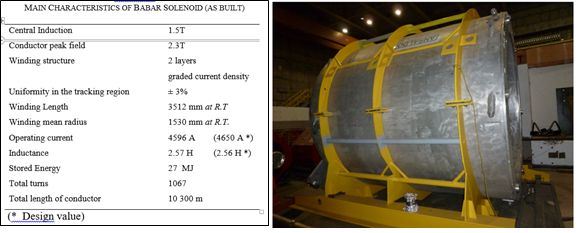
\includegraphics[width=0.9\textwidth]{figs/BaBar_Stats.png}
    \caption{}
    \label{fig:BaBarStats}
\end{figure}

\subsection{Refurbishment of the BaBar Solenoid}

The re-use of the magnet has been the subject of a engineering study and risk analysis, available as an EIC Technical Note (EICTJ-O-DE-PLT-TD-0017-R00), which also details the potential actions required to refurbish the BaBar solenoid for use in ECCE. 